\documentclass{jlreq}

\usepackage{titlesec}
\usepackage{listings}
\usepackage{fancyhdr}

% url
\usepackage{url}

% \adjustbox
\usepackage{adjustbox}

% tcolorboxの設定
\usepackage[most]{tcolorbox} 
\tcbuselibrary{breakable}
\tcbuselibrary{skins}
\tcbuselibrary{listingsutf8}
% タイトルのフォーマットを変更
\titleformat{\title}
  {\centering\Huge\bfseries}
  {}
  {0em} 
  {}

\titleformat{\subtitle}
  {\centering\Large\itshape}
  {}
  {0em}
  {}

\titleformat{\subsubsection}[block]
  {\normalfont\normalsize\bfseries}
  {\arabic{subsubsection}.}
  {1em}
  {}

\titleformat{\section}[block]
  {\normalfont\large\bfseries}
  {\Roman{section}.}
  {1em} 
  {}
  [\titleline{\titlerule[1pt]}]

\titleformat{\subsection}[block]
  {\normalfont\normalsize\bfseries}
  {\roman{subsection}.}
  {1em}
  {}

% listingsの設定

\renewcommand{\lstlistingname}{コード}

\lstset{
	breaklines = true,
	language = Python,
	keywordstyle = {\bfseries \color[cmyk]{0,1,0,0}},
	commentstyle = {\itshape \color[cmyk]{1,0.4,1,0}},
	numbers = left,
	numberstyle = \tiny,
	stepnumber = 1,
	% frameとnumberの間の距離
	numbersep = 10pt,
	frame = single,
	basicstyle = \ttfamily,
	tabsize = 2,
	captionpos = t,
	backgroundcolor={\color[gray]{.90}},
	showstringspaces = false,
}

% headerの設定
\pagestyle{fancy}
\fancyhf{}

\fancyhead[RO,RE]{\rightmark}
\fancyhead[LO,LE]{\leftmark} 
\fancyfoot[C]{\thepage}

% tikzの設定
\usepackage{tikz}

\begin{document}
探索の章で扱うアルゴリズムは以下と通りです。

\begin{itemize}
  \item 線形探索
  \item 二分探索
  \item 二分探索木
  \item Treeq
  \item 平衡木(AVL木、B木、赤黒木)
  \item ハッシュ法
\end{itemize}

検索(サーチ)とは、データ集合(配列など)から、目的とする値を持った要素を探し出すことを意味する。

\section{線形探索}

\textbf{線形探索}は、目的とする要素が見つかるまで先頭から順に要素を見ていく探索方法です。例えば、以下の配列で0を探すなら前から順番に、
8, 4, 5, 0, 2の順に要素を見ていきます。

\vspace{0.5cm}

\begin{center}
  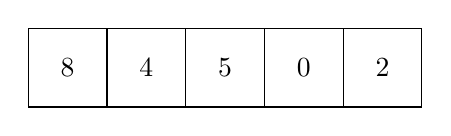
\begin{tikzpicture}
      \draw (0, 0) rectangle (1, 1);
      \node at (0.5, 0.5) {8};
      
      \draw (1, 0) rectangle (2, 1);
      \node at (1.5, 0.5) {4};
      
      \draw (2, 0) rectangle (3, 1);
      \node at (2.5, 0.5) {5};
      
      \draw (3, 0) rectangle (4, 1);
      \node at (3.5, 0.5) {0};
      
      \draw (4, 0) rectangle (5, 1);
      \node at (4.5, 0.5) {2};
  \end{tikzpicture}
\end{center}

\subsection{線形探索の実装}
\begin{lstlisting}[caption=線形探索の実装, frame=TRBL, label={linear}]
def linear_search(array: list[int], value: int) -> int:
    """
    線形探索をして一致するならそのindexを返す. 一致しないときは-1を返す
    """
    for i in range(len(array)):
        if array[i] == value:
            return i
    
    return -1


\end{lstlisting}

\subsection{番兵}

番兵法では探索するデータ集合の最後に目的とする数を追加します。最後に番兵を追加することで、より効率的に探索を行うことができます。
実際には番兵を追加してもそこまで効率が良くなるわけではないですが、番兵を追加することで、ループの条件判定を省略することができます。

\vspace{0.5cm}

\begin{center}
  \begin{tikzpicture}
      \draw (0, 0) rectangle (1, 1);
      \node at (0.5, 0.5) {8};
      
      \draw (1, 0) rectangle (2, 1);
      \node at (1.5, 0.5) {4};
      
      \draw (2, 0) rectangle (3, 1);
      \node at (2.5, 0.5) {5};
      
      \draw (3, 0) rectangle (4, 1);
      \node at (3.5, 0.5) {3};
      
      \draw (4, 0) rectangle (5, 1);
      \node at (4.5, 0.5) {2};
      
      \draw (5, 0) rectangle (6, 1);
      \fill[red, overlay] (5, 0) rectangle (6, 1);
      \node[white] at (5.5, 0.5) {0};
      \node[] at (5.5, -0.5) {番兵};
  \end{tikzpicture}
\end{center}

\begin{lstlisting}[caption=番兵の実装, frame=TRBL, label={sentinel}]
def linear_search(array: list[int], value: int) -> int:
    """
    線形探索をして一致するならそのindexを返す. 一致しないときは-1を返す
    """
    i = 0
    copied_array = array.copy()
    copied_array.append(value)
    while copied_array[i] != value: i += 1
    
    return i if i < len(array) else -1
  \end{lstlisting}

\section{二分探索}

\subsection{配列を探索する二分探索}

二分探索はソートされた配列に対して高速に探索を行うアルゴリズムの一つです。二分探索では探索する区間が条件に応じてどんどん半分になっていくため、
計算量は$O(\log n)$となります。以下の配列に対して、二分探索で18を探す場合を考えましょう。

最初の区間は配列全体を取ります。0-indexedな配列を考えると、midは39となり目的の18より大きいです。midが目的の値より大きい場合、
右の区間を狭めます。right = mid - 1とします。

\vspace{0.5cm}

\begin{center}
  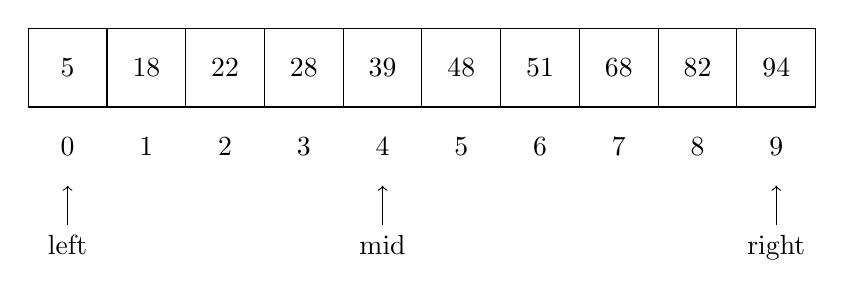
\begin{tikzpicture}
      \draw (0, 0) rectangle (1, 1);
      \node at (0.5, 0.5) {5};
      
      \draw (1, 0) rectangle (2, 1);
      \node at (1.5, 0.5) {18};
      
      \draw (2, 0) rectangle (3, 1);
      \node at (2.5, 0.5) {22};
      
      \draw (3, 0) rectangle (4, 1);
      \node at (3.5, 0.5) {28};
      
      \draw (4, 0) rectangle (5, 1);
      \node at (4.5, 0.5) {39};
      
      \draw (5, 0) rectangle (6, 1);
      \node at (5.5, 0.5) {48};
      
      \draw (6, 0) rectangle (7, 1);
      \node at (6.5, 0.5) {51};
      
      \draw (7, 0) rectangle (8, 1);
      \node at (7.5, 0.5) {68};
      
      \draw (8, 0) rectangle (9, 1);
      \node at (8.5, 0.5) {82};
      
      \draw (9, 0) rectangle (10, 1);
      \node at (9.5, 0.5) {94};

      \foreach \i in {0,1,...,9} {
        \node at (\i+0.5, -0.5) {\i};
    }

      % ラベルをはる
      \draw[<-] (0.5, -1) -- (0.5, -1.5) node[below] {left};
      \draw[<-] (9.5, -1) -- (9.5, -1.5) node[below] {right};
      \draw[<-] (4.5, -1) -- (4.5, -1.5) node[below] {mid};
  \end{tikzpicture}
\end{center}

\vspace{0.5cm}

rightを3に更新しました。mid = (0 + 3) // 2 = 1となります。midの値は18で目的の値と一致します。

\vspace{0.5cm}

\begin{center}
  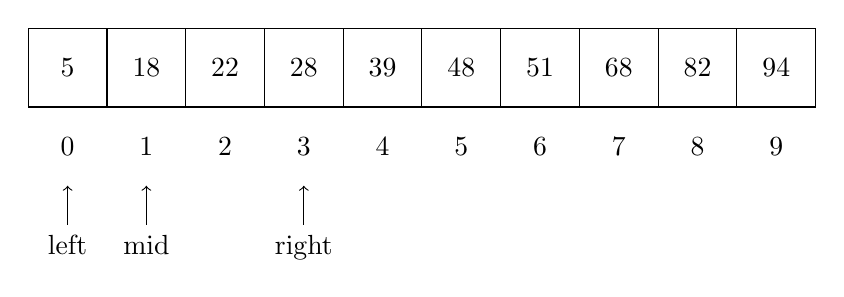
\begin{tikzpicture}
      \draw (0, 0) rectangle (1, 1);
      \node at (0.5, 0.5) {5};
      
      \draw (1, 0) rectangle (2, 1);
      \node at (1.5, 0.5) {18};
      
      \draw (2, 0) rectangle (3, 1);
      \node at (2.5, 0.5) {22};
      
      \draw (3, 0) rectangle (4, 1);
      \node at (3.5, 0.5) {28};
      
      \draw (4, 0) rectangle (5, 1);
      \node at (4.5, 0.5) {39};
      
      \draw (5, 0) rectangle (6, 1);
      \node at (5.5, 0.5) {48};
      
      \draw (6, 0) rectangle (7, 1);
      \node at (6.5, 0.5) {51};
      
      \draw (7, 0) rectangle (8, 1);
      \node at (7.5, 0.5) {68};
      
      \draw (8, 0) rectangle (9, 1);
      \node at (8.5, 0.5) {82};
      
      \draw (9, 0) rectangle (10, 1);
      \node at (9.5, 0.5) {94};

      \foreach \i in {0,1,...,9} {
        \node at (\i+0.5, -0.5) {\i};
    }

      % ラベルをはる
      \draw[<-] (0.5, -1) -- (0.5, -1.5) node[below] {left};
      \draw[<-] (1.5, -1) -- (1.5, -1.5) node[below] {mid};
      \draw[<-] (3.5, -1) -- (3.5, -1.5) node[below] {right};
  \end{tikzpicture}
\end{center}

\vspace{0.5cm}

次に、目的とする値を19として配列に存在しない場合を考えましょう。mid = 1の値は18で目的の値よりも小さいので、下の図のようにleftをmid + 1に更新します。
mid = (2 + 3) // 2 = 2となります。midの値は22で目的の値より大きいです。よって、rightをmid - 1に更新します。
すると、right = 1, left = 2となり、left > rightとなるので探索を終了します。

\vspace{0.5cm}

\begin{center}
  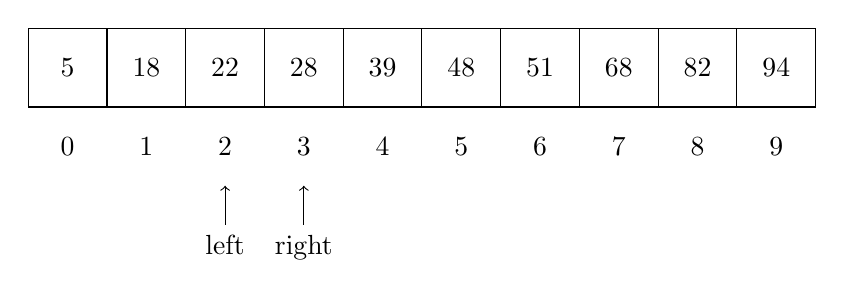
\begin{tikzpicture}
      \draw (0, 0) rectangle (1, 1);
      \node at (0.5, 0.5) {5};
      
      \draw (1, 0) rectangle (2, 1);
      \node at (1.5, 0.5) {18};
      
      \draw (2, 0) rectangle (3, 1);
      \node at (2.5, 0.5) {22};
      
      \draw (3, 0) rectangle (4, 1);
      \node at (3.5, 0.5) {28};
      
      \draw (4, 0) rectangle (5, 1);
      \node at (4.5, 0.5) {39};
      
      \draw (5, 0) rectangle (6, 1);
      \node at (5.5, 0.5) {48};
      
      \draw (6, 0) rectangle (7, 1);
      \node at (6.5, 0.5) {51};
      
      \draw (7, 0) rectangle (8, 1);
      \node at (7.5, 0.5) {68};
      
      \draw (8, 0) rectangle (9, 1);
      \node at (8.5, 0.5) {82};
      
      \draw (9, 0) rectangle (10, 1);
      \node at (9.5, 0.5) {94};

      \foreach \i in {0,1,...,9} {
        \node at (\i+0.5, -0.5) {\i};
    }

      % ラベルをはる
      \draw[<-] (2.5, -1) -- (2.5, -1.5) node[below] {left};
      \draw[<-] (3.5, -1) -- (3.5, -1.5) node[below] {right};
  \end{tikzpicture}
\end{center}

二分探索の実装は以下の通りです。

\begin{lstlisting}[caption=二分探索の実装, frame=TRBL, label={simle_binary}]
def binary_search(A: list[int], value: int) -> int:
    left, right = 0, len(A) - 1
    
    while left <= right:
        mid = (left + right) // 2
        
        if A[mid] == value:
            return mid
        
        if A[mid] < value:
            left = mid + 1
        else:
            right = mid - 1
    
    return -1
\end{lstlisting}

\subsection{一般化した二分探索}
Pythonの標準ライブラリであるbisectのbisect\_leftの実装をしましょう。bisect\_leftはソートされた配列に対して、
与えられた値以上の最小のindexを返す関数です。bisect\_leftは二分探索を用いて実装されています。先ほどの配列から要素を探す二分探索では、要素一致するか否かを判定していましたが、
今回はもっと一般化して「midがある条件を満たすか否か」を判定して範囲を狭めていきます。このとき、leftより右側の区間は
条件を満たさず、rightより左側の区間は条件を満たすようにします。 



\vspace{0.5cm}

\begin{center}
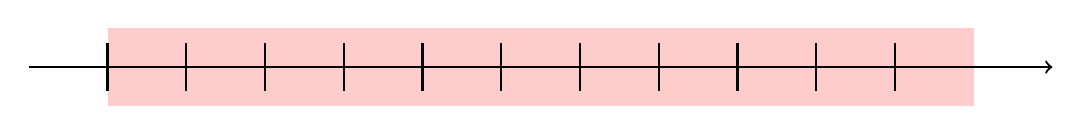
\begin{tikzpicture}
    \fill[red!20] (1, 0.5) rectangle (12, 1.5);
    \foreach \x in {1, 2, 3, 4, 5, 6, 7, 8, 9, 10, 11} {
        \draw[thick] (\x, 0.7) -- (\x, 1.3);
    }

    \draw[->, thick] (0, 1) -- (13, 1);
\end{tikzpicture}
\end{center}

\newpage

\section{参考}
\textbf{二分探索}

\begin{itemize}
  \item \url{https://qiita.com/drken/items/97e37dd6143e33a64c8c}
\end{itemize}


\end{document}